\let\negmedspace\undefined
\let\negthickspace\undefined
\documentclass[journal]{IEEEtran}
\usepackage[a5paper, margin=10mm, onecolumn]{geometry}
%\usepackage{lmodern} % Ensure lmodern is loaded for pdflatex
\usepackage{tfrupee} % Include tfrupee package

\setlength{\headheight}{1cm} % Set the height of the header box
\setlength{\headsep}{0mm}     % Set the distance between the header box and the top of the text

\usepackage{gvv-book}
\usepackage{gvv}
\usepackage{cite}
\usepackage{amsmath,amssymb,amsfonts,amsthm}
\usepackage{algorithmic}
\usepackage{graphicx}
\usepackage{textcomp}
\usepackage{xcolor}
\usepackage{txfonts}
\usepackage{listings}
\usepackage{enumitem}
\usepackage{mathtools}
\usepackage{gensymb}
\usepackage{comment}
\usepackage[breaklinks=true]{hyperref}
\usepackage{tkz-euclide} 
\usepackage{listings}
\def\inputGnumericTable{}                                 
\usepackage[latin1]{inputenc}                                
\usepackage{color}                                            
\usepackage{array}                                            
\usepackage{longtable}                                       
\usepackage{calc}                                             
\usepackage{multirow}                                         
\usepackage{hhline}                                           
\usepackage{ifthen}                                           
\usepackage{lscape}
\begin{document}

\bibliographystyle{IEEEtran}


\title{4.8.8}
\author{AI25BTECH11012 - GARIGE UNNATHI}
% \maketitle
% \newpage
% \bigskip
{\let\newpage\relax\maketitle}


\renewcommand{\thefigure}{\theenumi}
\renewcommand{\thetable}{\theenumi}
\setlength{\intextsep}{10pt} % Space between text and floats


\numberwithin{equation}{enumi}
\numberwithin{figure}{enumi}

\vspace{-1cm}

\textbf{Question}:\\
Find the equation of the plane passing through the point (-1,3,2) and perpendicular
to the planes x + 2y + 3z = 5 and 3x + 3y + z = 0. .


\textbf{Solution: }

 

The equation of a plane can be given by the formula :
         
\begin{align*}
    \mathbf{n^{T}}\vec{x} = c
\end{align*}
From the above formula we can write :
\begin{align}
  x + 2y + 3z = 5  = \myvec{1\\2\\3}^{T}\vec{x} = 5\\
  3x + 3y + z = 0  = \myvec{3\\3\\1}^{T}\vec{x} = 0
\end{align}

\begin{table}[h!]    
      \centering
      \documentclass{beamer}
\usepackage[utf8]{inputenc}

\usetheme{Madrid}
\usecolortheme{default}
\usepackage{amsmath,amssymb,amsfonts,amsthm}
\usepackage{txfonts}
\usepackage{tkz-euclide}
\usepackage{listings}
\usepackage{adjustbox}
\usepackage{array}
\usepackage{tabularx}
\usepackage{gvv}
\usepackage{lmodern}
\usepackage{circuitikz}
\usepackage{tikz}
\usepackage{graphicx}
\usepackage{multicol}
\setbeamertemplate{page number in head/foot}[totalframenumber]

\usepackage{tcolorbox}
\tcbuselibrary{minted,breakable,xparse,skins}



\definecolor{bg}{gray}{0.95}
\DeclareTCBListing{mintedbox}{O{}m!O{}}{%
  breakable=true,
  listing engine=minted,
  listing only,
  minted language=#2,
  minted style=default,
  minted options={%
    linenos,
    gobble=0,
    breaklines=true,
    breakafter=,,
    fontsize=\small,
    numbersep=8pt,
    #1},
  boxsep=0pt,
  left skip=0pt,
  right skip=0pt,
  left=25pt,
  right=0pt,
  top=3pt,
  bottom=3pt,
  arc=5pt,
  leftrule=0pt,
  rightrule=0pt,
  bottomrule=2pt,

  colback=bg,
  colframe=orange!70,
  enhanced,
  overlay={%
    \begin{tcbclipinterior}
    \fill[orange!20!white] (frame.south west) rectangle ([xshift=20pt]frame.north west);
    \end{tcbclipinterior}},
  #3,
}
\lstset{
    language=C,
    basicstyle=\ttfamily\small,
    keywordstyle=\color{blue},
    stringstyle=\color{orange},
    commentstyle=\color{green!60!black},
    numbers=left,
    numberstyle=\tiny\color{gray},
    breaklines=true,
    showstringspaces=false,
}
%------------------------------------------------------------
%This block of code defines the information to appear in the
%Title page
\title %optional
{5.13.38}
\date{October  2025}
%\subtitle{A short story}

\author % (optional)
{BEERAM MADHURI - EE25BTECH11012}



\begin{document}


\frame{\titlepage}
\begin{frame}{Question}
Let $\mathbf{X}$ and $\mathbf{Y}$ be two arbitrary, $3 \times 3$, non-zero, skew-symmetric matrices and $\mathbf{Z}$ be an arbitrary $3 \times 3$, non-zero, symmetric matrix. Then which of the following matrices is (are) skew symmetric?

\begin{enumerate}
\begin{multicols}{4}
    \item $\mathbf{Y}^3 \mathbf{Z}^4 - \mathbf{Z}^4 \mathbf{Y}^3$
    \item $\mathbf{X}^{44} + \mathbf{Y}^{44}$
    \item $\mathbf{X}^4 \mathbf{Z}^3 - \mathbf{Z}^3 \mathbf{X}^4$
    \item $\mathbf{X}^{23} + \mathbf{Y}^{23}$
\end{multicols}
\end{enumerate}

\end{frame}
 
\begin{frame}{solution}
\frametitle{finding Skew Symmetric Matrices:}
Given,
\begin{align}
\begin{aligned}\vec{X}^\top &= -\vec{X} \quad (\text{Skew-Symmetric}) \\\vec{Y}^\top &= -\vec{Y} \quad (\text{Skew-Symmetric}) \\\vec{Z^\top} &= \vec{Z} \quad (\text{Symmetric})\end{aligned}
\end{align}
\end{frame}
\begin{frame}
Checking all options:\\
a) $\vec{Y^3 Z^4} - \vec{Z^4 Y^3}$\\
Let 
\begin{align}
A = \vec{Y^3 Z^4} - \vec{Z^4 Y^3}\\
A^\top &= (\vec{Y^3 Z^4} - \vec{Z^4 Y^3})^\top \\
A^\top &= (\vec{Y^3 Z^4})^\top - (\vec{Z^4 Y^3})^\top \\
A^\top &= (\vec{Z}^\top)^4 (\vec{Y}^\top)^3 - (\vec{Y}^\top)^3 (\vec{Z}^\top)^4 \\
A^\top &= (\vec{Z}^\top)^4 (\vec{Y}^\top)^3 - (\vec{Y}^\top)^3 (\vec{Z}^\top)^4\end{align}
\end{frame}
\begin{frame}
Now, substitute the given properties ($\vec{Z}^\top= \vec{Z}$ and $\vec{Y}^\top = -\vec{Y}$):
\begin{align}A^\top &= (\vec{Z})^4 (-\vec{Y})^3 - (-\vec{Y})^3 (\vec{Z})^4 \\
\text{Since } (-\vec{Y})^3 &= (-1)^3 \vec{Y}^3 = -\vec{Y}^3, \text{ we get:} \\
A^\top &= \vec{Z}^4 (-\vec{Y}^3) - (-\vec{Y}^3) \vec{Z}^4 \\
A^\top &= -\vec{Z}^4 \vec{Y}^3 + \vec{Y}^3 \vec{Z}^4 \\
A^\top &= \vec{Y}^3 \vec{Z}^4 - \vec{Z}^4 \vec{Y}^3\\
=\vec{A}\end{align}
Hence, $A$ is Symmetric Matrix.
\end{frame}
\begin{frame}
b) $\vec{X}^{44} + \vec{Y}^{44}$\\
Let 
\begin{align}
B = \vec{X}^{44} + \vec{Y}^{44}\\
B^\top = (\vec{X}^{44} + \vec{Y}^{44})^\top \\
B^\top = (\vec{X}^{44})^\top + (\vec{Y}^{44})^\top \\
B^\top = (\vec{X}^\top)^{44} + (\vec{Y}^\top)^{44}
\end{align}
\end{frame}
\begin{frame}
Now, substitute the given properties ($\vec{X}^\top = -\vec{X}$ and $\vec{Y}^\top = -\vec{Y}$):
\begin{align}
B^\top = (-\vec{X})^{44} + (-\vec{Y})^{44}\\
(-1)^{44} = 1 \\
\therefore (-\vec{X})^{44} = \vec{X}^{44} and (-\vec{Y})^{44} = \vec{Y}^{44} \\
B^\top = \vec{X}^{44} + \vec{Y}^{44}\\
B^\top=B
\end{align}
Hence, $B$ is Symmetric Matrix.
\end{frame}
\begin{frame}
c)  $\vec{X}^4\vec{Z}^3 - \vec{Z}^3\vec{X}^4$\\Let
\begin{align}
C&=(\vec{X^4Z^3} - \vec{Z^3X^4})\\
C^\top &= (\vec{X^4Z^3} - \vec{Z^3X^4})^\top \\
C^\top &= (\vec{X^4Z^3})^\top - (\vec{Z^3X^4})^\top \\
C^\top &= (\vec{Z}^3)^\top(\vec{X}^4)^\top - (\vec{X}^4)^\top(\vec{Z}^3)^\top \\
C^\top &= (\vec{Z}^\top)^3(\vec{X}^\top)^4 - (\vec{X}^\top)^4(\vec{Z}^\top)^3
\end{align}
\end{frame}
\begin{frame}
Now, substitute the given properties ($\vec{Z}^\top = \vec{Z}$ and $\vec{X}^\top = -\vec{X}$):
\begin{align}
C^\top&= (\vec{Z})^3(-\vec{X})^4 - (-\vec{X})^4(\vec{Z})^3 \\
(-\vec{X})^4 &= \vec{X}^4 \\
\vec{C}^\top &= \vec{Z}^3\vec{X}^4 - \vec{X}^4\vec{Z}^3 \\
C^\top &= -(\vec{X}^4\vec{Z}^3 - \vec{Z}^3\vec{X}^4)\\
=-C
\end{align}
Hence, $C$ is Skew Symmetric Matrix.
\end{frame}
\begin{frame}
d) $\vec{X^{23} + Y}^{23}$\\Let
\begin{align}
D&=\vec{X}^{23} + \vec{Y}^{23}\\
D^\top &= (\vec{X}^{23} + \vec{Y}^{23})^\top \\
D^\top &= (\vec{X}^{23})^\top + (\vec{Y}^{23})^\top \\
D^\top &= (\vec{X}^\top)^{23} + (\vec{Y}^\top)^{23}
\end{align}
\end{frame}
\begin{frame}
Now, substitute the given properties ($\vec{X}^\top = -\vec{X}$ and $\vec{Y}^\top = -\vec{Y}$):
\begin{align}
D^\top &= (-\vec{X})^{23} + (-\vec{Y})^{23} \\
(-1)^{23} = -1\\
(-\vec{X})^{23} = -\vec{X}^{23} \text{ and } (-\vec{Y})^{23} = -\vec{Y}^{23}\\
D^\top &= -\vec{X}^{23} - \vec{Y}^{23} \\
D^\top &= -(\vec{X}^{23} + \vec{Y}^{23})\\
=-D
\end{align}
Hence, $D$ is Skew Symmetric Matrix.
\end{frame}
\begin{frame}
$\therefore$ Option 3. $\vec{X}^4\vec{Z}^3 - \vec{Z}^3\vec{X}^4$ and\\ 
Option 4. $\vec{X^{23} + Y}^{23}$ are Skew Symmetric
\end{frame}

\begin{frame}[fragile]
\frametitle{Python Code}
\begin{lstlisting}
import numpy as np

# --- 1. Define Helper Functions ---
def is_skew_symmetric(matrix):
    """
    Checks if a matrix M is skew-symmetric by verifying if M^T = -M.
    Uses np.allclose for accurate floating-point comparisons.
    """
    return np.allclose(matrix.T, -matrix)
\end{lstlisting}
\end{frame}

\begin{frame}[fragile]
\frametitle{python Code}
\begin{lstlisting}
def is_symmetric(matrix):
    """Checks if a matrix M is symmetric by verifying if M^T = M."""
    return np.allclose(matrix.T, matrix)
# --- 2. Generate Arbitrary Non-Zero Matrices ---
# To create a skew-symmetric matrix, we can use the formula A - A^T
# To create a symmetric matrix, we can use the formula A + A^T

# Create a random 3x3 matrix to generate X
A = np.random.rand(3, 3)
X = A - A.T  # X is now skew-symmetric
\end{lstlisting}
\end{frame}

\begin{frame}[fragile]
\frametitle{python Code}
\begin{lstlisting}
# Create another random 3x3 matrix to generate Y
B = np.random.rand(3, 3)
Y = B - B.T  # Y is now skew-symmetric

# Create a random 3x3 matrix to generate Z
C = np.random.rand(3, 3)
Z = C + C.T  # Z is now symmetric
\end{lstlisting}
\end{frame}

\begin{frame}[fragile]
\frametitle{python Code}
\begin{lstlisting}
# --- 3. Verify Properties of Generated Matrices ---
print("--- Initial Matrix Properties ---")
print(f"Is X skew-symmetric? {is_skew_symmetric(X)}")
print(f"Is Y skew-symmetric? {is_skew_symmetric(Y)}")
print(f"Is Z symmetric?      {is_symmetric(Z)}")
print("-" * 35)

# Note: @ is the operator for matrix multiplication in NumPy
M_a = np.linalg.matrix_power(Y, 3) @ np.linalg.matrix_power(Z, 4) - \
      np.linalg.matrix_power(Z, 4) @ np.linalg.matrix_power(Y, 3)
print(f"a) Is Y³Z⁴ - Z⁴Y³ skew-symmetric?  {is_skew_symmetric(M_a)}")
\end{lstlisting}
\end{frame}

\begin{frame}[fragile]
\frametitle{python Code}
\begin{lstlisting}
# b) X^44 + Y^44
M_b = np.linalg.matrix_power(X, 44) + np.linalg.matrix_power(Y, 44)
print(f"b) Is X⁴⁴ + Y⁴⁴ skew-symmetric?      {is_skew_symmetric(M_b)}")

# c) X^4 * Z^3 - Z^3 * X^4
M_c = np.linalg.matrix_power(X, 4) @ np.linalg.matrix_power(Z, 3) - \
      np.linalg.matrix_power(Z, 3) @ np.linalg.matrix_power(X, 4)
\end{lstlisting}
\end{frame}

\begin{frame}[fragile]
\frametitle{python Code}
\begin{lstlisting}
print(f"c) Is X⁴Z³ - Z³X⁴ skew-symmetric?  {is_skew_symmetric(M_c)}")

# d) X^23 + Y^23
M_d = np.linalg.matrix_power(X, 23) + np.linalg.matrix_power(Y, 23)
print(f"d) Is X²³ + Y²³ skew-symmetric?      {is_skew_symmetric(M_d)}")
print("-" * 35)
\end{lstlisting}
\end{frame}

\begin{frame}[fragile]
\frametitle{C Code}
\begin{lstlisting}
#include <stdio.h>
#include <math.h>
#include <string.h>
#define N 3
void print_matrix(const char* name, double mat[N][N]) {
    printf("Matrix %s:\n", name);
    for (int i = 0; i < N; i++) {
        for (int j = 0; j < N; j++) {
            printf("%9.2f ", mat[i][j]);
        }
        printf("\n");
    }
    printf("\n");
}
\end{lstlisting}
\end{frame}

\begin{frame}[fragile]
\frametitle{C Code}
\begin{lstlisting}
// Multiplies two 3x3 matrices: C = A * B
void multiply_matrices(double a[N][N], double b[N][N], double c[N][N]) {
    for (int i = 0; i < N; i++) {
        for (int j = 0; j < N; j++) {
            c[i][j] = 0;
            for (int k = 0; k < N; k++) {
                c[i][j] += a[i][k] * b[k][j];
            }
        }
    }
}
\end{lstlisting}
\end{frame}

\begin{frame}[fragile]
\frametitle{C Code}
\begin{lstlisting}
// Calculates matrix power: result = mat^p
void power_matrix(double mat[N][N], int p, double result[N][N]) {
    // Initialize result as identity matrix
    for (int i = 0; i < N; i++) {
        for (int j = 0; j < N; j++) {
            result[i][j] = (i == j) ? 1.0 : 0.0;
        }
    }    
    double temp[N][N];
    for (int i = 0; i < p; i++) {
        multiply_matrices(result, mat, temp);
        memcpy(result, temp, sizeof(double) * N * N);
    }
}
\end{lstlisting}
\end{frame}

\begin{frame}[fragile]
\frametitle{C Code}
\begin{lstlisting}
// Adds two matrices: C = A + B
void add_matrices(double a[N][N], double b[N][N], double c[N][N]) {
    for (int i = 0; i < N; i++) {
        for (int j = 0; j < N; j++) {
            c[i][j] = a[i][j] + b[i][j];
        }
    }
}
\end{lstlisting}
\end{frame}

\begin{frame}[fragile]
\frametitle{C Code}
\begin{lstlisting}
// Subtracts two matrices: C = A - B
void subtract_matrices(double a[N][N], double b[N][N], double c[N][N]) {
    for (int i = 0; i < N; i++) {
        for (int j = 0; j < N; j++) {
            c[i][j] = a[i][j] - b[i][j];
        }
    }
}
\end{lstlisting}
\end{frame}

\begin{frame}[fragile]
\frametitle{C Code}
\begin{lstlisting}
// Checks if a matrix is skew-symmetric (M^T = -M)
int is_skew_symmetric(double mat[N][N]) {
    const double epsilon = 1e-9; // Tolerance for float comparison
    for (int i = 0; i < N; i++) {
        for (int j = 0; j < N; j++) {
            // Check if M[i][j] is approximately -M[j][i]
            if (fabs(mat[i][j] + mat[j][i]) > epsilon) {
                return 0; // Not skew-symmetric
            }
        }
    }
\end{lstlisting}
\end{frame}

\begin{frame}[fragile]
\frametitle{C Code}
\begin{lstlisting}
    // Check if diagonal elements are zero
    for (int i = 0; i < N; i++) {
        if (fabs(mat[i][i]) > epsilon) {
            return 0; // Not skew-symmetric
        }
    }
    return 1; // It is skew-symmetric
}
\end{lstlisting}
\end{frame}

\begin{frame}[fragile]
\frametitle{C Code}
\begin{lstlisting}
int main() {
    // Define arbitrary non-zero matrices as per the problem statement
    // X and Y are skew-symmetric (M[i][j] = -M[j][i])
    double X[N][N] = {
        {0.0, 1.0, 2.0},
        {-1.0, 0.0, 3.0},
        {-2.0, -3.0, 0.0}
    };
    double Y[N][N] = {
        {0.0, -2.0, 4.0},
        {2.0, 0.0, -5.0},
        {-4.0, 5.0, 0.0}
    };
\end{lstlisting}
\end{frame}

\begin{frame}[fragile]
\frametitle{C Code}
\begin{lstlisting}    
    // Z is symmetric (M[i][j] = M[j][i])
    double Z[N][N] = {
        {1.0, 2.0, 3.0},
        {2.0, 4.0, 5.0},
        {3.0, 5.0, 6.0}
    };
    // Temporary matrices for calculations
    double term1[N][N], term2[N][N], result[N][N];
    // --- Option (a): Y^3 * Z^4 - Z^4 * Y^3 ---
    power_matrix(Y, 3, term1);
    power_matrix(Z, 4, term2);
    double Y3Z4[N][N];
    multiply_matrices(term1, term2, Y3Z4);
\end{lstlisting}
\end{frame}

\begin{frame}[fragile]
\frametitle{C Code}
\begin{lstlisting} 
    power_matrix(Z, 4, term1);
    power_matrix(Y, 3, term2);
    double Z4Y3[N][N];
    multiply_matrices(term1, term2, Z4Y3);

    subtract_matrices(Y3Z4, Z4Y3, result);
    printf("a) Y^3*Z^4 - Z^4*Y^3 is skew-symmetric? --> %s\n", is_skew_symmetric(result) ? "Yes" : "No");
\end{lstlisting}
\end{frame}

\begin{frame}[fragile]
\frametitle{C Code}
\begin{lstlisting}
    // --- Option (b): X^44 + Y^44 ---
    power_matrix(X, 44, term1);
    power_matrix(Y, 44, term2);
    add_matrices(term1, term2, result);
    printf("b) X^44 + Y^44 is skew-symmetric? --> %s\n", is_skew_symmetric(result) ? "Yes" : "No");

    // --- Option (c): X^4 * Z^3 - Z^3 * X^4 ---
    power_matrix(X, 4, term1);
    power_matrix(Z, 3, term2);
    double X4Z3[N][N];
    multiply_matrices(term1, term2, X4Z3);
\end{lstlisting}
\end{frame}

\begin{frame}[fragile]
\frametitle{C Code}
\begin{lstlisting}
    power_matrix(Z, 3, term1);
    power_matrix(X, 4, term2);
    double Z3X4[N][N];
    multiply_matrices(term1, term2, Z3X4);
    
    subtract_matrices(X4Z3, Z3X4, result);
    printf("c) X^4*Z^3 - Z^3*X^4 is skew-symmetric? --> %s\n", is_skew_symmetric(result) ? "Yes" : "No");
\end{lstlisting}
\end{frame}

\begin{frame}[fragile]
\frametitle{C Code}
\begin{lstlisting}
    // --- Option (d): X^23 + Y^23 ---
    power_matrix(X, 23, term1);
    power_matrix(Y, 23, term2);
    add_matrices(term1, term2, result);
    printf("d) X^23 + Y^23 is skew-symmetric? --> %s\n", is_skew_symmetric(result) ? "Yes" : "No");
    printf("\n------------------------------------------------------\n")
    printf("Conclusion: The correct options are (c) and (d).\n");

    return 0;
}
\end{lstlisting}
\end{frame}

\begin{frame}[fragile]
\frametitle{Python and C Code}
\begin{lstlisting}
from ctypes import c_double
# Create a 3x3 matrix using ctypes
def create_matrix():
    return [[c_double(0.0) for _ in range(3)] for _ in range(3)]

# Example usage
mat = create_matrix()
mat[0][0] = c_double(1.0)
print(mat[0][0].value)

\end{lstlisting}
\end{frame}


\end{document}
      \caption{Variables Used}
      \label{}
    \end{table}


Let us assume the equation of the plane to be

\begin{align}
      \mathbf{n^{T}}\vec{x} = 1\\
      or \\
      \mathbf{x^{T}}\vec{n} = 1
\end{align}

As point $\vec{A}$ lies on the plane we can write :
\begin{align}
    \mathbf{A^{T}}\vec{n} = 1
\end{align}

If two planes are perpendicular then there normal vectors must also be perpendicular ,using this we can write :
\begin{align}
    \mathbf{n_1^{T}}\vec{n} = 0\\
    \mathbf{n_2^{T}}\vec{n} = 0
\end{align}

Combining equations 0.6,0.7 and 0.8 ,we get :
\begin{align}
    \mathbf{(A\quad n_1\quad n_2)^{T}}\vec{n} = \myvec{-1 & 3& 2\\
                                                      1 & 2 & 3\\
                                                      3 & 3& 1}\vec{n} = \myvec{1\\0\\0}
\end{align}
Solving the above equation by row reduction we get :
\begin{align}
    \vec{n} = \myvec{-\frac{7}{25} \\ \frac{8}{25} \\ -\frac{3}{25}} = \frac{1}{25}\myvec{-7\\8\\-3}
\end{align}

From the equation 0.3 we can write the plane euation as :
\begin{align}
    \myvec{-7\\8\\-3}^{T}\vec{x} = 25
\end{align}

\begin{figure}[h!]
   \centering
   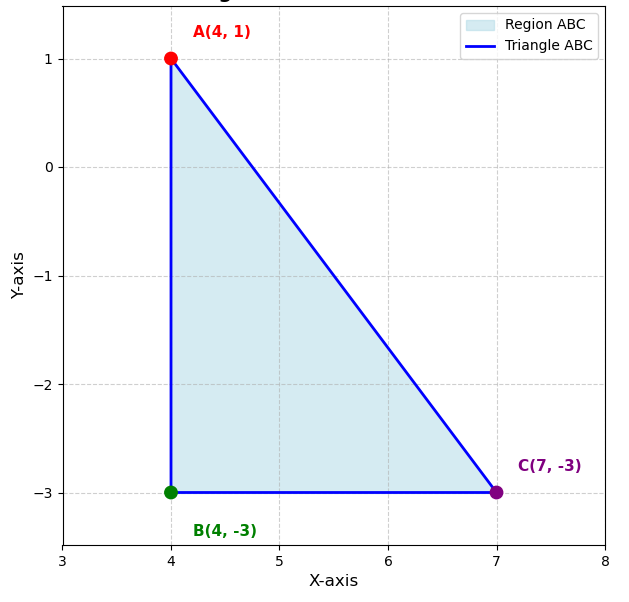
\includegraphics[width=0.7\linewidth]{/Users/unnathi/Documents/ee1030-2025/ai25btech11012/matgeo/4.8.8/figs/fig.png}
   \caption{}
   \label{stemplot}
\end{figure}


\end{document}



